\begin{center}
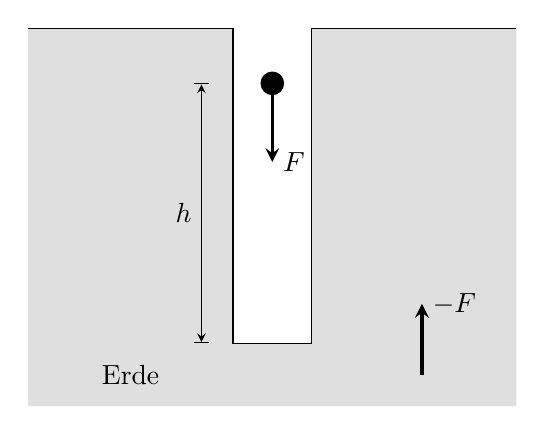
\begin{tikzpicture}[>=stealth]
 \fill[gray!25] (0,0) rectangle (2.6,4) (3.6,0) rectangle (6.2,4) (0,-0.8) rectangle (6.2,0);
 \draw (0,4) -- (2.6,4) -- (2.6,0) -- (3.6,0) -- (3.6,4) -- (6.2,4);
 \fill (3.1,3.3) circle (0.15);
 \draw[->, very thick] (3.1,3.15) -- (3.1,2.3) node[right] {$F$};
 \draw[->, very thick] (5,-0.4) -- (5,0.5) node[right] {$-F$};
 \node at (1.3,-0.4) {Erde};
 \draw[|<->|] (2.2,0) -- (2.2,3.3) node[midway, left] {$h$};
\end{tikzpicture}
\end{center}

\begin{abcliste}
\abc Der Impulserhaltungssatz gilt nur für ein abgeschlossenes System. Der Stein allein ist kein abgeschlossenes System: Die Gewichtskraft $F$ ist eine Kraft, die die Erde auf ihn ausübt. Nach dem Wechselwirkungsgesetz zieht der Stein die Erde mit der Gegenkraft $-F$ an. Im abgeschlossenen System Stein und Erde erhält die Erde deshalb in jedem Moment einen gleich grossen, entgegengesetzt gerichteten Impuls; der Gesamtimpuls bleibt null.

\abc Mit $g = \gEO$ erreicht der Stein am Boden die Geschwindigkeit und den Impuls
\begin{align}
 v &= \vStF = \sqrt{2\cdot\gE\cdot\hBr} = \vSt \\
 p &= \pStF = \mSt\cdot\vSt = \pSt
\end{align}
Die Erde hat bis dahin denselben Impuls nach oben aufgenommen. Beim Aufprall kommen Stein und Erde zur Ruhe, der Gesamtimpuls bleibt null. Die Geschwindigkeit der Erde ($M_\text{E} = \mEaO$, FoTaBe S.~209) ändert sich dabei um
\begin{align}
 \Delta v_\text{E} &= \frac{p}{M_\text{E}} = \vEaF \\
   &= \frac{\pSt}{\mEa} \\
   &= \vEa \approx \result{\vEaP{0}{2}}
\end{align}
Diese Geschwindigkeit ist unmessbar klein: Die Erde bleibt praktisch in Ruhe und kann als unbewegliche Unterlage betrachtet werden. Ihr Impuls ist trotzdem so gross wie der des Steins, weil ihre Masse riesig ist.
\end{abcliste}
